In this section, we describe the first steps you need to do to start
using FDPS\describeForIF{and FDPS \progLangName interface}. We explain the environment (the supported operating systems), the necessary software (compilers etc), and how to compile and run the sample codes.

%%%%%%%%%%%%%%%%%%%%%%%%%%%%%%%%%%%%%%%%%%%%%%%%%%%%%%%%%%%%%%%%
\subsection{Environment}
FDPS works on Linux, Mac OS X, Windows (with Cygwin). 


%%%%%%%%%%%%%%%%%%%%%%%%%%%%%%%%%%%%%%%%%%%%%%%%%%%%%%%%%%%%%%%%
\subsection{Necessary software}
In this section, we describe software necessary to use FDPS, first for standard functions, and then for extensions. 

%%%%%%%%%%%%%%%%%%%%%%%%%%%%%%%%
\subsubsection{Standard functions}
we describe software necessary to use standard functions of FDPS. First for the case of single-thread execution, then for multithread, then for multi-nodes.

%%%%%%%%%%%%%%%%
\subsubsubsection{Single thread}
\begin{itemize}
\item make
\item A C++ compiler (We have tested with gcc version 4.8.3 and  K
  compiler version 1.2.0)
\ifFtn % for Fortran doc.
\item A Fortran compiler that supports Fortran 2003 Standard and that are interoperable with the above C++ compiler (We have tested with gcc version 4.8.3).
\item Python 2.7.5 or later, or, Python 3.4 or later (correct operation is not guaranteed for older Python versions)
\endifFtn
\ifC % for C doc.
\item A C compiler that are interoperable with the above C++ compiler (We have tested with gcc version 4.8.3).
\item Python 2.7.5 or later, or, Python 3.4 or later (correct operation is not guaranteed for older Python versions)
\endifC
\end{itemize}

%%%%%%%%%%%%%%%%
\subsubsubsection{Parallel processing}
%%%%%%%%
\subsubsubsubsection{OpenMP}
\begin{itemize}
\item make
\item A C++ compiler with OpenMP support (We have tested with gcc version 4.8.3 and K compiler version 1.2.0)
\ifFtn % for Fortran doc.
\item A Fortran compiler with OpenMP support (it must support Fortran 2003 Standard and be interoperable with the above C++ compiler. We have tested with gcc version 4.8.3).
\item Python 2.7.5 or later, or, Python 3.4 or later (correct operation is not guaranteed for older Python versions)
\endifFtn
\ifC % for C doc.
\item A C compiler with OpenMP support (it must be interoperable with the above C++ compiler. We have tested with gcc version 4.8.3).
\item Python 2.7.5 or later, or, Python 3.4 or later (correct operation is not guaranteed for older Python versions)
\endifC
\end{itemize}

%%%%%%%%
\subsubsubsubsection{MPI}
\begin{itemize}
\item make
\item A C++ compiler which supports MPI version 1.3 or later. (We have
  tested with Open MPI 1.6.4 and K compiler version 1.2.0)
\ifFtn % for Fortran doc.
\item A Fortran compiler which supports MPI version 1.3 or later (it also must support Fortran 2003 Standard and be interoperable with the above C++ compiler. We have tested with OpenMPI 1.6.4).
\item Python 2.7.5 or later, or, Python 3.4 or later (correct operation is not guaranteed for older Python versions)
\endifFtn
\ifC % for C doc.
\item A C compiler which supports MPI version 1.3 or later (it also must be interoperable with the above C++ compiler. We have tested with OpenMPI 1.6.4).
\item Python 2.7.5 or later, or, Python 3.4 or later (correct operation is not guaranteed for older Python versions)
\endifC
\end{itemize}

%%%%%%%%
\subsubsubsubsection{MPI+OpenMP}
\begin{itemize}
\item make
\item A C++ compiler which supports OpenMP and MPI version 1.3 or later. (We have tested with Open MPI 1.6.4 and K compiler version 1.2.0)
\ifFtn % for Fortran doc.
\item A Fortran compiler which supports OpenMP and MPI version 1.3 or later (it also must support Fortran 2003 Standard and be interoperable with the above C++ compiler. We have tested with OpenMPI 1.6.4).
\item Python 2.7.5 or later, or, Python 3.4 or later (correct operation is not guaranteed for older Python versions)
\endifFtn
\ifC % for C doc.
\item A C compiler which supports OpenMP and MPI version 1.3 or later (it also must be interoperable with the above C++ compiler. We have tested with OpenMPI 1.6.4).
\item Python 2.7.5 or later, or, Python 3.4 or later (correct operation is not guaranteed for older Python versions)
\endifC
\end{itemize}

%%%%%%%%%%%%%%%%%%%%%%%%%%%%%%%%
\subsubsection{Extensions}
Current extension for FDPS is the ``Particle Mesh'' module.  We describe the necessary software for it below.

%%%%%%%%%%%%%%%%
\subsubsubsection{Particle Mesh}
\begin{itemize}
\item make
\item A C++ compiler which supports OpenMP and MPI version 1.3 or later. (We have tested with Open MPI 1.6.4)
\item FFTW 3.3 or later
\end{itemize}

%%%%%%%%%%%%%%%%%%%%%%%%%%%%%%%%%%%%%%%%%%%%%%%%%%%%%%%%%%%%%%%%
\subsection{Install}
In this section we describe how to get the FDPS software and how to build it.

%%%%%%%%%%%%%%%%%%%%%%%%%%%%%%%%
\subsubsection{How to get the software}
We first describe how to get the latest version, and then previous versions. We recommend to use the latest version.

%%%%%%%%%%%%%%%%
\subsubsubsection{The latest version}
You can use one of the following ways.
\begin{itemize}
\item Using browsers
\begin{enumerate}
\item Click ``Download ZIP'' in \url{https://github.com/FDPS/FDPS} to download \path{FDPS-master.zip}
\item Move the zip file to the directory under which you want to install FDPS and unzip the file (or place the files using some GUI).
\end{enumerate}
\item Using CLI (Command line interface)
\begin{itemize}
% When using SVN
\item Using Subversion:
\begin{screen}
\begin{verbatim}
$ svn co --depth empty https://github.com/FDPS/FDPS
$ cd FDPS
$ svn up trunk
\end{verbatim}
\end{screen}
% When using Git
\item Using Git
\begin{screen}
\begin{verbatim}
$ git clone git://github.com/FDPS/FDPS.git
\end{verbatim}
\end{screen}    
\end{itemize}
\end{itemize}

%%%%%%%%%%%%%%%%
\subsubsubsection{Previous versions}
You can get previous versions using browsers.
\begin{itemize}
\item Previous versions are listed in \url{https://github.com/FDPS/FDPS/releases}. Click the version you want to download it.
\item Extract the files under the directory you want.
\end{itemize}

%%%%%%%%%%%%%%%%%%%%%%%%%%%%%%%%
\subsubsection{How to install}
\describeForCpp{% C++ descriptions
There is no need for configure or setup. 
}
\describeForIF{% Fortran,C descriptions
Because FDPS is a header library\footnote{A library that consists of header files only.}, you do not have to execute the \texttt{configure} command. All you need to do is to expand the archive of FDPS in some directory and to setup the include PATH when you compile your codes. An actual procedures can be found in Makefiles of the sample codes explained in \S~\ref{subsec:how_to_comple_and_run_sample_codes}.

When using FDPS from \progLangName, you first must create interface programs to FDPS based on user's codes. Its procedure is described in Chap.~6 of the specification document \path{doc_spec_ftn_en.pdf}. Makefiles of the sample codes are written so that the interface programs are automatically generated when \texttt{make} are running. We recommend that users use Makefiles of the sample codes as a reference when making your own Makefile.
}

%%%%%%%%%%%%%%%%%%%%%%%%%%%%%%%%%%%%%%%%%%%%%%%%%%%%%%%%%%%%%%%%
\subsection{How to compile and run the sample codes}
\label{subsec:how_to_comple_and_run_sample_codes}
We provide two samples: one for gravitational $N$-body simulation and the other for SPH. We first describe gravitational $N$-body simulation and then SPH. Sample codes do not use extensions. 

%%%%%%%%%%%%%%%%%%%%%%%%%%%%%%%%
\subsubsection{Gravitational $N$-body simulation}
%%%%%%%%%%%%%%%%
\subsubsubsection{Summary}
Through the following steps one can use this sample.
\begin{itemize}
\item Move to the directory \dirNameNbodySample. Here, \texttt{\$(FDPS)} denotes the highest-level directory for FDPS (Note that \texttt{FDPS} is not an environmental variable). The actual value of \texttt{\$(FDPS)} depends on the way you acquire the software. If you used the browser, the last part is ``FDPS-master''. If you used Subversion or Git, it is ``trunk'' or ``FDPS'', respectively. 
\item Edit \texttt{Makefile} in the current directory (\dirNameNbodySample).
\item Run the \texttt{make} command to create the executable \texttt{nbody.out}.
\item Run \texttt{nbody.out}
\item Check the output.
\end{itemize}
In addition, we describe the way to use Phantom-GRAPE for x86.

%%%%%%%%%%%%%%%%
\subsubsubsection{Move to the directory with the sample code}
Move to \dirNameNbodySample.

%%%%%%%%%%%%%%%%
\subsubsubsection{Edit Makefile}
\label{s3sec:edit_Makefile_in_nbody}
\ifCpp % C++ description [start]
Edit Makefile following the description below. The changes depend on if you use OpenMP and/or MPI.
\endifCpp % C++ description [end]
\ifFtn % Fortran description [start]
In the directory, there are two Makefiles: \texttt{Makefile} and \texttt{Makefile.intel}. The former is for GCC and the latter is for the Intel compilers. In this section, we mainly describe \texttt{Makefile} in detail and give an usage note on \texttt{Makefile.intel} at the end of this section.

First, we describe the default setting of \texttt{Makefile}. There are four Makefile variables that need to be set when compiling the sample code. They are the following. \texttt{FC} that stores the command to run a Fortran compiler, \texttt{CXX} that stores the command to run a C++ compiler, and \texttt{FCFLAGS} and \texttt{CXXFLAGS}, in which compiler options for both compilers are stored. The initial values of these variables are as follows:
\begin{screen}
\begin{Verbatim}[commandchars=\\\{\}]
FC=gfortran
CXX=g++
FCFLAGS = -std=f2003 -O3 -ffast-math -funroll-loops -finline-functions
CXXFLAGS = -O3 -ffast-math -funroll-loops \$(FDPS_INC)
\end{Verbatim}
\end{screen}
where \texttt{\$(FDPS\_INC)} is the variable storing the include PATH for FDPS. It is already set in this Makefile and you do not need to modify it here.

An executable file can be obtained by executing the \texttt{make} command after setting the above four Makefile variables appropriately. Edit \texttt{Makefile} according the following descriptions. The changes depend on if you use OpenMP and/or MPI.
\endifFtn % Fortran description [end]
\ifC % C description [start]
In the directory, there is a Makefile for GCC, \texttt{Makefile}. In this section, we mainly describe this Makefile in detail.

First, we describe the default setting of \texttt{Makefile}. There are four Makefile variables that need to be set when compiling the sample code. They are the following. \texttt{CC} that stores the command to run a C compiler, \texttt{CXX} that stores the command to run a C++ compiler, and \texttt{CFLAGS} and \texttt{CXXFLAGS}, in which compiler options for both compilers are stored. The initial values of these variables are as follows:
\begin{screen}
\begin{Verbatim}[commandchars=\\\{\}]
CC=gcc
CXX=g++
CFLAGS = -O3 -ffast-math -funroll-loops -finline-functions
CXXFLAGS = -O3 -ffast-math -funroll-loops \$(FDPS_INC)
\end{Verbatim}
\end{screen}
where \texttt{\$(FDPS\_INC)} is the variable storing the include PATH for FDPS. It is already set in this Makefile and you do not need to modify it here.

An executable file can be obtained by executing the \texttt{make} command after setting the above four Makefile variables appropriately. Edit \texttt{Makefile} according the following descriptions. The changes depend on if you use OpenMP and/or MPI.
\endifC % C description [end]

\begin{itemize}  
%%% Without both OpenMP and MPI %%%
\item Without both OpenMP and MPI
\begin{itemize}
\ifCpp % C++ description
\item Set the variable \texttt{CC} the command to run your C++ compiler
\endifCpp
\ifFtn % Fortran description
\item Set the variable \texttt{FC} the command to run your Fortran compiler
\item Set the variable \texttt{CXX} the command to run your C++ compiler
\endifFtn
\ifC % C description
\item Set the variable \texttt{CC} the command to run your C compiler
\item Set the variable \texttt{CXX} the command to run your C++ compiler
\endifC
\end{itemize}
% With OpenMP but not with MPI  
\item With OpenMP but not with MPI
\begin{itemize}
\ifCpp % C++ descriptions
\item Set the variable \texttt{CC} the command to run your C++ compiler
\item Uncomment the line \texttt{CFLAGS += -DPARTICLE\_SIMULATOR\_THREAD\_PARALLEL -fopenmp}. If you use Intel compiler, replace \texttt{-fopenmp} by \texttt{-qopenmp} or \texttt{-openmp} depending on the version of the compiler.
\endifCpp
\ifFtn % Fortran descriptions
\item Set the variable \texttt{FC} the command to run your Fortran compiler with OpenMP support
\item Set the variable \texttt{CXX} the command to run your C++ compiler with OpenMP support
\item Uncomment the line \texttt{FCFLAGS += -DPARTICLE\_SIMULATOR\_THREAD\_PARALLEL -fopenmp}
\item Uncomment the line \texttt{CXXFLAGS += -DPARTICLE\_SIMULATOR\_THREAD\_PARALLEL -fopenmp}
\endifFtn
\ifC % C descriptions
\item Set the variable \texttt{CC} the command to run your C compiler with OpenMP support
\item Set the variable \texttt{CXX} the command to run your C++ compiler with OpenMP support
\item Uncomment the line \texttt{CFLAGS += -DPARTICLE\_SIMULATOR\_THREAD\_PARALLEL -fopenmp}
\item Uncomment the line \texttt{CXXFLAGS += -DPARTICLE\_SIMULATOR\_THREAD\_PARALLEL -fopenmp}
\endifC
\end{itemize}
% With MPI but not with OpenMP  
\item With MPI but not with OpenMP
\begin{itemize}
\ifCpp % C++ descriptions
\item Set the variable \texttt{CC} the command to run your MPI C++ compiler
\item Uncomment the line \texttt{CFLAGS += -DPARTICLE\_SIMULATOR\_MPI\_PARALLEL}
\endifCpp
\ifFtn % Fortran descriptions
\item Set the variable \texttt{FC} the command to run your Fortran compiler that supports MPI
\item Set the variable \texttt{CXX} the command to run your C++ compiler that supports MPI
\item Uncomment the line \texttt{FCFLAGS += -DPARTICLE\_SIMULATOR\_MPI\_PARALLEL}
\item Uncomment the line \texttt{CXXFLAGS += -DPARTICLE\_SIMULATOR\_MPI\_PARALLEL}
\endifFtn
\ifC % C descriptions
\item Set the variable \texttt{CC} the command to run your C compiler that supports MPI
\item Set the variable \texttt{CXX} the command to run your C++ compiler that supports MPI
\item Uncomment the line \texttt{CFLAGS += -DPARTICLE\_SIMULATOR\_MPI\_PARALLEL}
\item Uncomment the line \texttt{CXXFLAGS += -DPARTICLE\_SIMULATOR\_MPI\_PARALLEL}
\endifC
\end{itemize}
% With both OpenMP and MPI  
\item With both OpenMP and MPI
\begin{itemize}
\ifCpp % C++ description
\item Set the variable \texttt{CC} the command to run your MPI C++ compiler
\item Uncomment the line \texttt{CFLAGS += -DPARTICLE\_SIMULATOR\_THREAD\_PARALLEL -fopenmp}. If you use Intel compiler, replace \texttt{-fopenmp} by \texttt{-qopenmp} or \texttt{-openmp} depending on the version of the compiler.
  \item Uncomment the line \texttt{CFLAGS += -DPARTICLE\_SIMULATOR\_MPI\_PARALLEL}
\endifCpp
\ifFtn % Fortran description
\item Set the variable \texttt{FC} the command to run your Fortran compiler that supports both OpenMP and MPI
\item Set the variable \texttt{CXX} the command to run your C++ compiler that supports both OpenMP and MPI
\item Uncomment the line \texttt{FCFLAGS += -DPARTICLE\_SIMULATOR\_THREAD\_PARALLEL -fopenmp}
\item Uncomment the line \texttt{FCFLAGS += -DPARTICLE\_SIMULATOR\_MPI\_PARALLEL}
\item Uncomment the line \texttt{CXXFLAGS += -DPARTICLE\_SIMULATOR\_THREAD\_PARALLEL -fopenmp}
\item Un comment the line \texttt{CXXFLAGS += -DPARTICLE\_SIMULATOR\_MPI\_PARALLEL}
\endifFtn
\ifC % C description
\item Set the variable \texttt{CC} the command to run your C compiler that supports both OpenMP and MPI
\item Set the variable \texttt{CXX} the command to run your C++ compiler that supports both OpenMP and MPI
\item Uncomment the line \texttt{CFLAGS += -DPARTICLE\_SIMULATOR\_THREAD\_PARALLEL -fopenmp}
\item Uncomment the line \texttt{CFLAGS += -DPARTICLE\_SIMULATOR\_MPI\_PARALLEL}
\item Uncomment the line \texttt{CXXFLAGS += -DPARTICLE\_SIMULATOR\_THREAD\_PARALLEL -fopenmp}
\item Un comment the line \texttt{CXXFLAGS += -DPARTICLE\_SIMULATOR\_MPI\_PARALLEL}
\endifC
\end{itemize}
\end{itemize}

\ifFtn % Fortran description [start]
Next, we describe useful information when users use this Makefile to compile users' codes. Most important variables when using this Makefile are \texttt{FDPS\_LOC}, \texttt{SRC\_USER\_DEFINED\_TYPE}, and \texttt{SRC\_USER}. The variable \texttt{FDPS\_LOC} is used to store the PATH of the top directory of FDPS. Based on the value of \texttt{FDPS\_LOC}, this Makefile automatically sets a lot of variables related to FDPS, such as the PATH of the directory storing FDPS source files and the PATH of the Python script to generate Fortran interface. Thus, users should set appropriately. The variable \texttt{SRC\_USER\_DEFINED\_TYPE} is used to store a list of names of Fortran files in which user-defined types are implemented, while the variable \texttt{SRC\_USER} is used to store a list of names of Fortran files in which all the rest are implemented. The reason why we divide users' source files as above is to avoid needless recompilation of FDPS (as a result, we can reduce time required to compile and link users' codes): Because FDPS Fortran interface programs are generated based on user-defined types, we need to recompile of FDPS only when files specified by \texttt{SRC\_USER\_DEFINED\_TYPE} are modified. However, there is one thing users should be careful of. When there are dependencies between files specified by \texttt{SRC\_USER\_DEFINED\_TYPE} or \texttt{SRC\_USER}, users must describe these dependencies in Makefile. As for the way of describing dependencies in Makefile, please see the manual of GNU make, for example.

Finally, we describe the usage note for \texttt{Makefile.intel}. Except for the initial values of Makefile variables, \texttt{Makefile.intel} has the same structure as that of \texttt{Makefile}. Hence, users can make use of \texttt{Makefile.intel} in the same way as \texttt{Makefile} by modifying the values of the variables appropriately. The followings are things to keep in mind when editing Makefile:
\begin{itemize}[leftmargin=*]
\item \texttt{/opt/intel/bin} should be replaced by the PATH of a directory that stores Intel compilers in your computer system.
\item \texttt{/opt/intel/include} should be replaced by the PATH of a directory that stores header files used by Intel compilers.
\item By default, the value of the variable \texttt{LDFLAGS} is \texttt{-L/opt/intel/lib/intel64 -L/usr/lib64 -lifport -lifcore -limf -lsvml -lm -lipgo -lirc -lirc\_s}. Among them, the option \texttt{-lifcore} \footnote{\texttt{libifcore} is an Intel compiler's Fortran runtime library.} is necessary for the Intel C++ compiler to link C++ objects and Fortran objects\footnote{We have tested this with Intel compilers (ver. 17.0.0 20160721).}. When the Intel compiler's libraries are not in the library PATH of the system, users need to specify libraries as \texttt{-L/opt/intel/lib/intel64 -L/usr/lib64 -lifport -limf -lsvml -lm -lipgo -lirc -lirc\_s}, where \texttt{/opt/intel/lib/intel64} is the PATH of directory that stores the Intel compiler's libraries, \texttt{/usr/lib64} is the PATH of directory storing the library \texttt{libm}. These PATHs depend on the systems users use and therefore users must modify these appropriately. Note that libraries required to compile users' codes (\texttt{-l*}) may change depending on the version of Intel compilers and please confirm these.
\item As of writing this (2016/12/26), the compile option that invokes OpenMP support is either \texttt{-openmp} or \texttt{-qopenmp} depending the version of Intel compilers. Recent compilers use the latter option (if the former is specified in this case, the compiler issues a waring of ``deprecated'').
\item Depending on computer systems, all of the necessary settings except for the specification of the option \texttt{-lifcore} may be done by environment variables such as \texttt{PATH}, \texttt{CPATH}, \texttt{LD\_LIBRARY\_PATH}.
\end{itemize}
\endifFtn % Fortran description [end]
\ifC % C description [start]
Next, we describe useful information when users use this Makefile to compile users' codes. Most important variables when using this Makefile are \texttt{FDPS\_LOC}, \texttt{HDR\_USER\_DEFINED\_TYPE}, and \texttt{SRC\_USER}. The variable \texttt{FDPS\_LOC} is used to store the PATH of the top directory of FDPS. Based on the value of \texttt{FDPS\_LOC}, this Makefile automatically sets a lot of variables related to FDPS, such as the PATH of the directory storing FDPS source files and the PATH of the Python script to generate C interface. Thus, users should set appropriately. The variable \texttt{HDR\_USER\_DEFINED\_TYPE} is used to store a list of names of C header files in which user-defined types are implemented, while the variable \texttt{SRC\_USER} is used to store a list of names of C files in which all the rest are implemented. The reason why we divide users' source files as above is to avoid needless recompilation of FDPS (as a result, we can reduce time required to compile and link users' codes): Because FDPS C interface programs are generated based on user-defined types, we need to recompile of FDPS only when files specified by \texttt{HDR\_USER\_DEFINED\_TYPE} are modified. However, there is one thing users should be careful of. When there are dependencies between files specified by \texttt{HDR\_USER\_DEFINED\_TYPE} or \texttt{SRC\_USER}, users must describe these dependencies in Makefile. As for the way of describing dependencies in Makefile, please see the manual of GNU make, for example.
\endifC

%%%%%%%%%%%%%%%%
\subsubsubsection{Run make}
Type ``make'' to run \texttt{make}.
\describeForIF{ % Fortran,C description
In the process of \texttt{make}, \progLangName interface programs are first generated and then they are compiled together with the sample codes.
}


%%%%%%%%%%%%%%%%
\subsubsubsection{Run the sample code}
\begin{itemize}
\item If you are not using MPI, run the following in CLI (terminal)
\begin{screen}
\begin{verbatim}
$ ./nbody.out
\end{verbatim}
\end{screen}
  
\item If you are using MPI, run the following in CLI (terminal)
\begin{screen}
\begin{verbatim}
$ MPIRUN -np NPROC ./nbody.out
\end{verbatim}
\end{screen}
Here, \texttt{MPIRUN} should be \texttt{mpirun} or \texttt{mpiexec} depending on your MPI configuration, and \texttt{NPROC} is the number of processes you will use.

Upon normal completion, the following output log should appear in stderr. The exact value of the energy error may depend on the system, but it is okay if its absolute value is of the order of $1 \times 10^{-3}$.
\ifCpp %C++
\begin{screen}
\begin{verbatim}
time:  9.6250000 energy error: -4.512836e-03
time:  9.7500000 energy error: -4.440746e-03
time:  9.8750000 energy error: -4.652358e-03
time: 10.0000000 energy error: -4.605855e-03
MemoryPool::finalize() is completed!
******** FDPS has successfully finished. ********
\end{verbatim}
\end{screen}
\endifCpp
\ifFtn %Fortran
\begin{screen}
\begin{verbatim}
time:    9.5000000000E+000, energy error:   -3.8046534069E-003
time:    9.6250000000E+000, energy error:   -3.9711750200E-003
time:    9.7500000000E+000, energy error:   -3.8223429428E-003
time:    9.8750000000E+000, energy error:   -3.8843099298E-003
MemoryPool::finalize() is completed!
******** FDPS has successfully finished. ********
\end{verbatim}
\end{screen}
\endifFtn
\ifC % C
\begin{screen}
\begin{verbatim}
time:      7.000, energy error:  -3.8957312e-03
time:      8.000, energy error:  -3.7788873e-03
time:      9.000, energy error:  -3.7627744e-03
time:     10.000, energy error:  -3.7071071e-03
MemoryPool::finalize() is completed!
******** FDPS has successfully finished. ********
\end{verbatim}
\end{screen}
\endifC
\end{itemize}

%%%%%%%%%%%%%%%%
\subsubsubsection{Analysis of the result}
In the directory \texttt{result},
\describeForCpp{% for C++
files ``000x.dat'' have been created. These files store the distribution of particles. Here, x is an integer (from 0 to 9) and it indicates time.
}
\describeForIF{% for Fortran,C
files ``snap0000x-proc0000y.dat'' have been created. These files store the distribution of particles. Here, x is an integer indicating time and y is an integer indicating MPI process number (y is always 0 if the program is executed without MPI).
}
The output file format is that in each line, index of particle, mass, position (x, y, z) and velocity (vx, vy, vz) are listed.

What is simulated with the default sample is the cold collapse of an uniform sphere with radius three expressed using 1024 particles. Using gnuplot, you can see the particle distribution in the xy plane at time=9:

\ifCpp % for C++用
\begin{screen}
\begin{verbatim}
$ gnuplot
$ plot "result/0009.dat" using 3:4
\end{verbatim}
\end{screen}
\endifCpp
\ifIF % for Fortran,C
\begin{screen}
\begin{verbatim}
$ cd result
$ cat snap00009-proc* > snap00009.dat
$ gnuplot
> plot "snap00009.dat" using 3:4
\end{verbatim}
\end{screen}
\endifIF

By plotting the particle distributions at other times, you can see
how the initially uniform sphere contracts and then expands again.
(Figure \ref{fig:nbody}).

\begin{figure}
\begin{center}
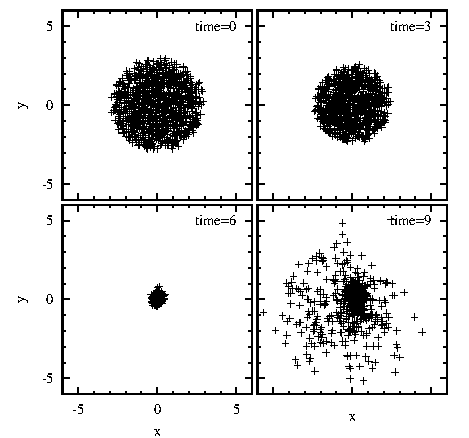
\includegraphics[width=0.75\linewidth]{fig/nbody.pdf}
\end{center}
\caption{}
\label{fig:nbody}
\end{figure}

\ifCpp % for C++
To increase the number of particles to $10000$, try:
(without MPI)
\begin{screen}
\begin{verbatim}
$ ./nbody.out -N 10000
\end{verbatim}
\end{screen}
\endifCpp
\ifIF % for Fortran, C 
To increate the number of particles to $10000$, set the value of the parameter variable \texttt{ntot} (defined in the \procedure \mainFuncName in the file \fileNameOfMainFunc) to $10000$, then recompile the sample codes, and run the executable file again.
\endifIF



%%%%%%%%%%%%%%%%
\subsubsubsection{To use Phantom-GRAPE for x86}
\label{s3sec:phantom_grape_x86}
If you are using a computer with Intel or AMD x86 CPU, you can use Phantom-GRAPE for x86.

Move to the directory \texttt{\$(FDPS)/src/phantom\_grape\_x86/G5/newton/libpg5}, edit the Makefile there (if necessary), and run make to build the Phantom-GRAPE library \texttt{libpg5.a}.

Then go back to directory \dirNameNbodySample, edit Makefile and remove ``\#'' at the top of the line \\''\#use\_phantom\_grape\_x86 = yes'', and (after removing the existing executable) run make again. (Same for with and without OpenMP or MPI). You can run the executable in the same way as that for the executable without Phantom GRAPE.

The performance test on a machine with Intel Core i5-3210M CPU @2.50GHz (2 cores, 4 threads) indicates that, for N=8192, the code with Phantom GRAPE is faster than that without Phantom GRAPE by a factor a bit less than five.

\ifCpp % for C++
The following is the sample command line:
\begin{screen}
\begin{verbatim}
$ ./nbody.out -N 8192 -n 256
\end{verbatim}
\end{screen}
\endifCpp

%%%%%%%%%%%%%%%%
\subsubsubsection{To use PIKG}
\label{s3sec:pikg}
PIKG (\url{https://github.com/FDPS/PIKG}) is a tool to generate a highly-optimized, two-body inter-particle interaction calculation kernel for particle simulations from a simple description of the interaction using a DSL (Domain Specific Language).

In order to use kernels generated by PIKG, open Makefile in directory \\
\dirNameNbodySample\  and remove \texttt{\#} at the top of the line \texttt{\#use\_pikg\_x86 = yes}. Then, (after removing the existing executable) run
\describeForEach{ % C++
\texttt{make pikg}.
}{ %Fortran
\texttt{make}.
}{% C
\texttt{make}.
}
(Same for with and without OpenMP or MPI). You can run the executable in the same way as that for the executable without PIKG.

In the default, PIKG generates kernels in \texttt{reference} mode. In this mode, unoptimized kernels are generated. To generate kernels optimized for specific architectures such as AVX2 and AVX-512, change \texttt{CONVERSION\_TYPE} in Makefile and remove \texttt{\#} at the top of the line containing \texttt{*FLAGS} (where \texttt{*} is the usual regular expression symbol). 

%%%%%%%%%%%%%%%%
\ifCpp % C++
\subsubsubsection{To use NVIDIA GPUs}
\label{sec:use_nvidia_gpu}

The sample program includes the interaction kernel written in Cuda for NVIDIA GPUs.

Uncomment the line ``\#use\_cuda\_gpu = yes'' in file \texttt{Makefile} in \dirNameNbodySample and assign to  CUDA\_HOME in Makefile  a value appropriate to your environment. You can then run  make to obtain the executable (OpenMP and MPI are also supported). The executable can be tested in the same way as the non-GPU version.
\endifCpp

%%%%%%%%%%%%%%%%%%%%%%%%%%%%%%%%
\subsubsection{SPH simulation code}
%%%%%%%%%%%%%%%%
\subsubsubsection{Summary}
Through the following steps one can use this sample.
\begin{itemize}
\item Move to the directory \dirNameSPHSample.
\item Edit Makefile in the current directory (\dirNameSPHSample).
\item Run make command to create the executable \texttt{sph.out}.
\item Run \texttt{sph.out}.
\item Check the output.
\end{itemize}

%%%%%%%%%%%%%%%%
\subsubsubsection{Move to the directory with the sample code}
Move to \dirNameSPHSample.

%%%%%%%%%%%%%%%%
\subsubsubsection{Edit Makefile}
Edit Makefile following the same description described in \S~\ref{s3sec:edit_Makefile_in_nbody}.

%%%%%%%%%%%%%%%%
\subsubsubsection{Run make}
Type ``make'' to run \texttt{make}.
\describeForIF{% for Fortran, C
As in $N$-body sample code, in the process of \texttt{make}, \progLangName interface programs are first generated. Then, they are compiled together with SPH sample codes.
}

%%%%%%%%%%%%%%%%
\subsubsubsection{Run the sample code}
\begin{itemize}
\item If you are not using MPI, run the following in CLI (terminal)
\begin{screen}
\begin{verbatim}
$ ./sph.out
\end{verbatim}
\end{screen}
  
\item If you are using MPI, run the following in CLI (terminal)
\begin{screen}
\begin{verbatim}
$ MPIRUN -np NPROC ./sph.out
\end{verbatim}
\end{screen}
\end{itemize}
Here, \texttt{MPIRUN} should be \texttt{mpirun} or \texttt{mpiexec} depending on your MPI configuration, and \texttt{NPROC} is the number of processes you will use.

Upon normal completion, the following output log should appear in stderr. 
\begin{screen}
\begin{verbatim}
******** FDPS has successfully finished. ********
\end{verbatim}
\end{screen}

%%%%%%%%%%%%%%%%
\subsubsubsection{Analysis of the result}
In the directory \texttt{result},
\describeForCpp{% for C++
files ``000x.txt'' have been created. These files store the distribution of particles. Here, x is an integer (from 0 to 9) and it indicates time.
}
\describeForIF{% for Fortran and C
files ``snap0000x-proc0000y.dat'' have been created. These files store the distribution of particles. Here, x and y are integers that indicate time and MPI process number, respectively. When executing the program without MPI, y is always 0.
}
The output file format is that in each line, index of particle, mass, position (x, y, z), velocity (vx, vy, vz), density, internal energy and pressure are listed.

What is simulated is the three-dimensional shock-tube problem. Using gnuplot, you can see the plot of the x-coordinate and density of particles at time=40:
\ifCpp % for C++
\begin{screen}
\begin{verbatim}
$ gnuplot
$ plot "result/0040.txt" using 3:9
\end{verbatim}
\end{screen}
\endifCpp
\ifIF % for Fortran and C
\begin{screen}
\begin{verbatim}
$ cd result
$ cat snap00040-proc* > snap00040.dat
$ gnuplot
> plot "snap00040.dat" using 3:9
\end{verbatim}
\end{screen}
\endifIF

When the sample worked correctly, a figure similar to Figure \ref{fig:sph} should appear.
\begin{figure}
\begin{center}
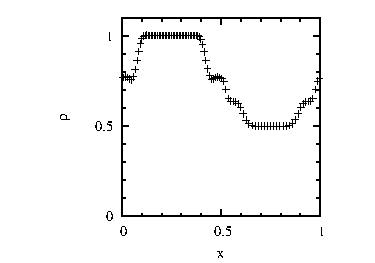
\includegraphics[width=0.5\linewidth]{fig/sph.pdf}
\end{center}
\caption{}
\label{fig:sph}
\end{figure}
